%! TEX root = ../main.tex
\documentclass[main]{subfiles}

\begin{document}
\chapter{結果・考察}

以下に設定すべき変数を示す.
\begin{table}[ht]
    \centering
    \caption{シミュレーションに使用する変数}
    \begin{tabular}{ll}
        \toprule
        変数       & 意味         \\
        \midrule
        $T$      & シミュレーション時間 \\
        $u$      & 流体の初期速度    \\
        $length$ & 物体の長さ      \\
        $width$  & 物体の幅       \\
        $\nu$    & 動せん断粘度     \\
        $\rho$   & 密度         \\
        \bottomrule
    \end{tabular}%
    \label{tab:result-variables}%
\end{table}

以下特に指定しない限り,
$\nu=\SI{1.48E-5}{\square\meter\per\second}$,
$\rho=\SI{1.225}{\kilogram\per\cubic\meter}$とする.
\footnote{
    実際,シミュレーションではLBM単位系を用いる.
    FluidX3Dでは,SI単位系とLBM単位系とで変換を行う関数が用意されているため,SI単位系で設定をすれば十分.
}

次に,実験をしたモデルを示す.

\begin{itemize}
    \item Formula1 Mercedes W14 \footnote{https://downloadfree3d.com/3d-models/vehicles/sports-car/mercedes-f1-w14/}
    \item Space Shuttle \footnote{https://www.thingiverse.com/thing:4975964/files}
    \item Ahmed Bluff Body \footnote{https://github.com/nathanrooy/ahmed-bluff-body-cfd}
\end{itemize}

\clearpage
\section{物体の周りの気流の流れの可視化}
\subsection{Formula1 Mercedes W14}
フリーのMercedes F1 W14モデル
\footnote{
    実際のFormula 1には全部で10チーム20台のマシンが参加しておりそれぞれ異なるが,
    大まかな形状は同じである.
}
を使用して,$u=\SI{100}{\kilo\meter\per\hour}$とし,
実験をした結果の一部を以下\ref{fig:result-f1}に示す.
\footnote{
    実験の動画は以下のリンクから視聴できる.
    \url{https://youtu.be/rhfD4j8yjgk}
    \url{https://youtu.be/dGVB6DQThHI}
}
\footnote{
    FluidX3Dのバグとして,突然流体の速度が無限大に発散してしまうものが報告されている.
    \url{https://github.com/ProjectPhysX/FluidX3D/issues/109}.

    実際,次の動画のように,この実験でも突然流体の速度が無限大に発散してしまうことがあった.
    \url{https://youtu.be/PRkXo401tNI}.
    そのため本実験では,抗力・揚力の計算は行うことができなかった.

}



\begin{figure}[htbp]
    \begin{tabular}{cc}
        \begin{minipage}[b]{0.45\linewidth}
            \centering
            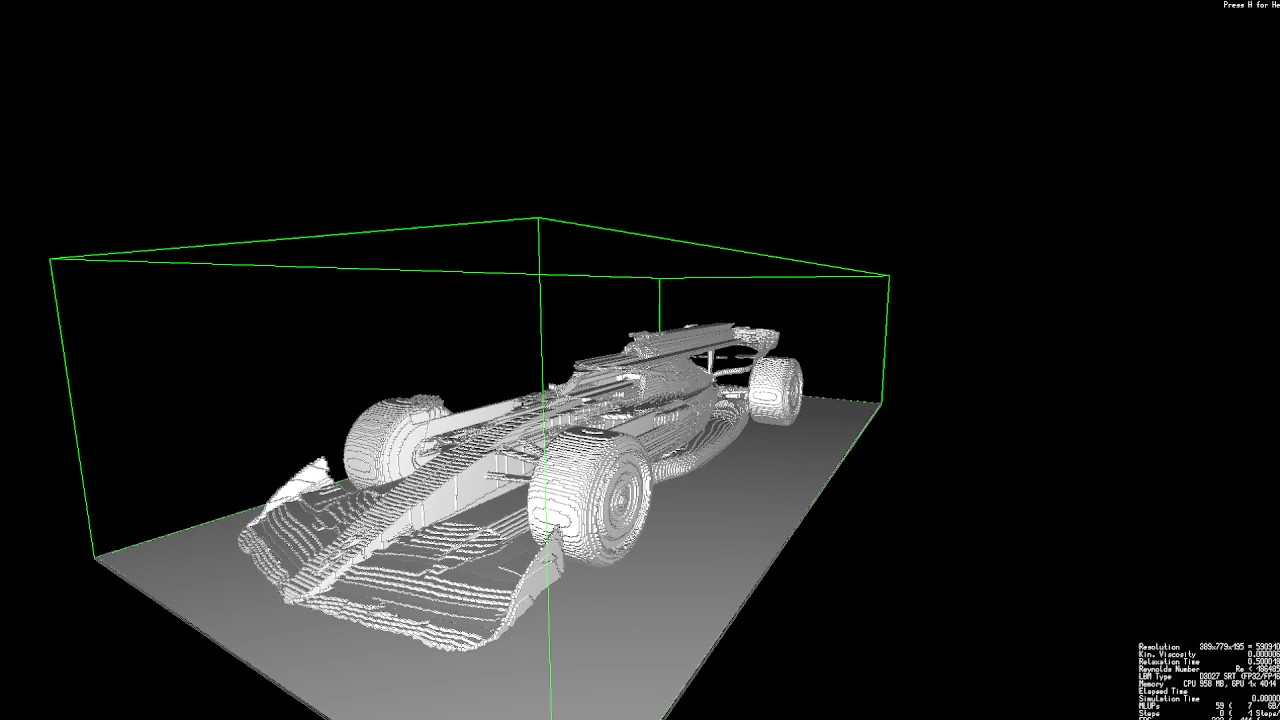
\includegraphics[width=0.9\linewidth]{figures/f1/2023-11-05 13-13-52 - frame at 0m0s.jpg}
            \subcaption{\SI{0}{\second}}
        \end{minipage}  &
        \begin{minipage}[b]{0.45\linewidth}
            \centering
            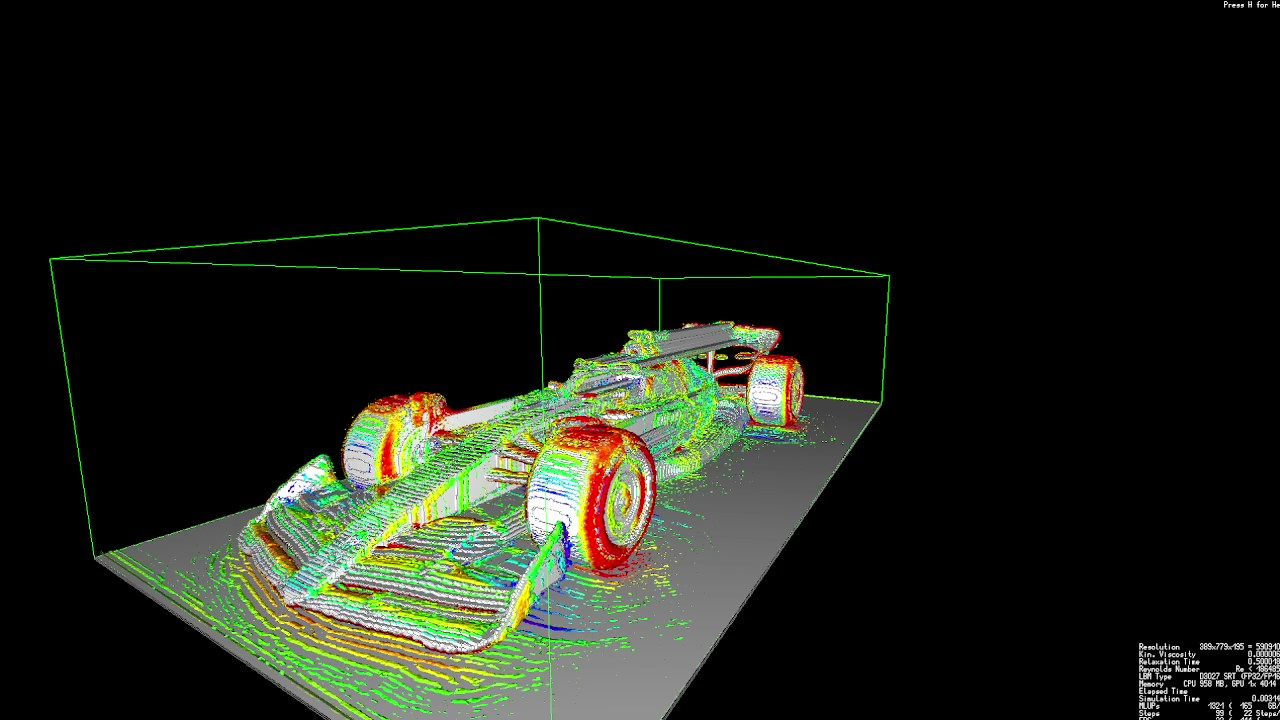
\includegraphics[width=0.9\linewidth]{figures/f1/2023-11-05 13-13-52 - frame at 0m7s.jpg}
            \subcaption{\SI{7}{\second}}
        \end{minipage}  \\
        \begin{minipage}[b]{0.45\linewidth}
            \centering
            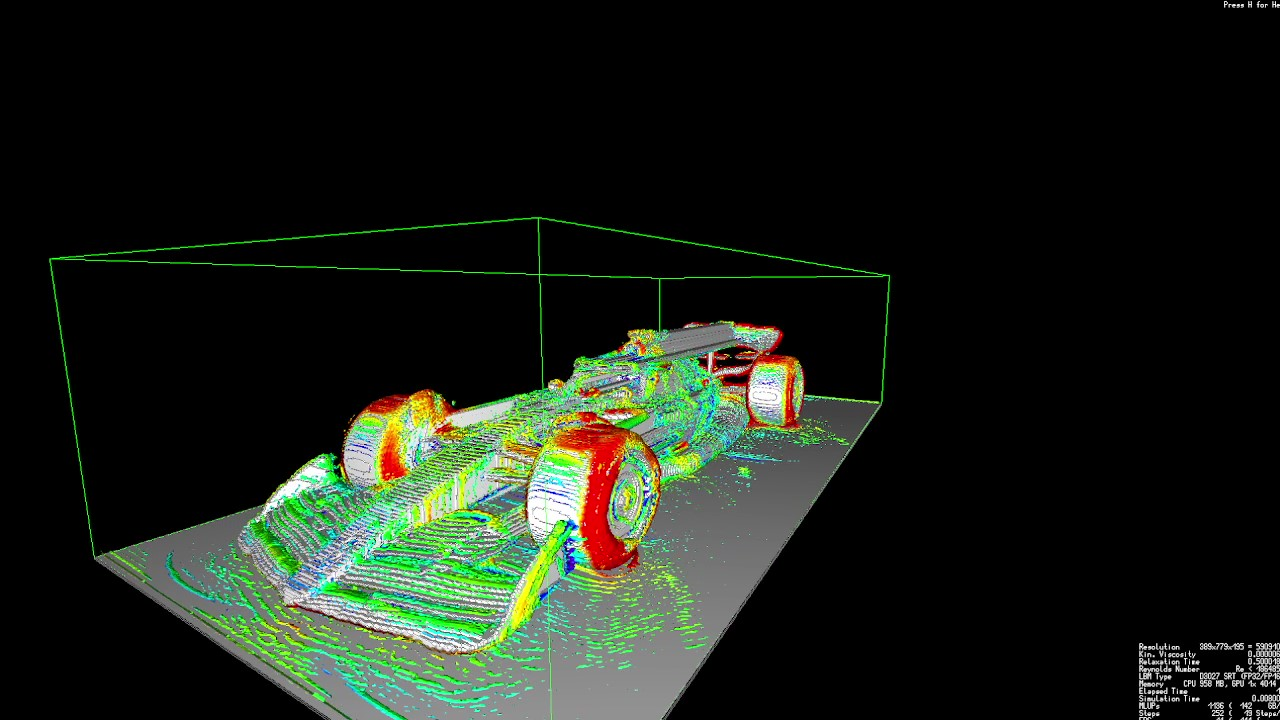
\includegraphics[width=0.9\linewidth]{figures/f1/2023-11-05 13-13-52 - frame at 0m14s.jpg}
            \subcaption{\SI{14}{\second}}
        \end{minipage} &
        \begin{minipage}[b]{0.45\linewidth}
            \centering
            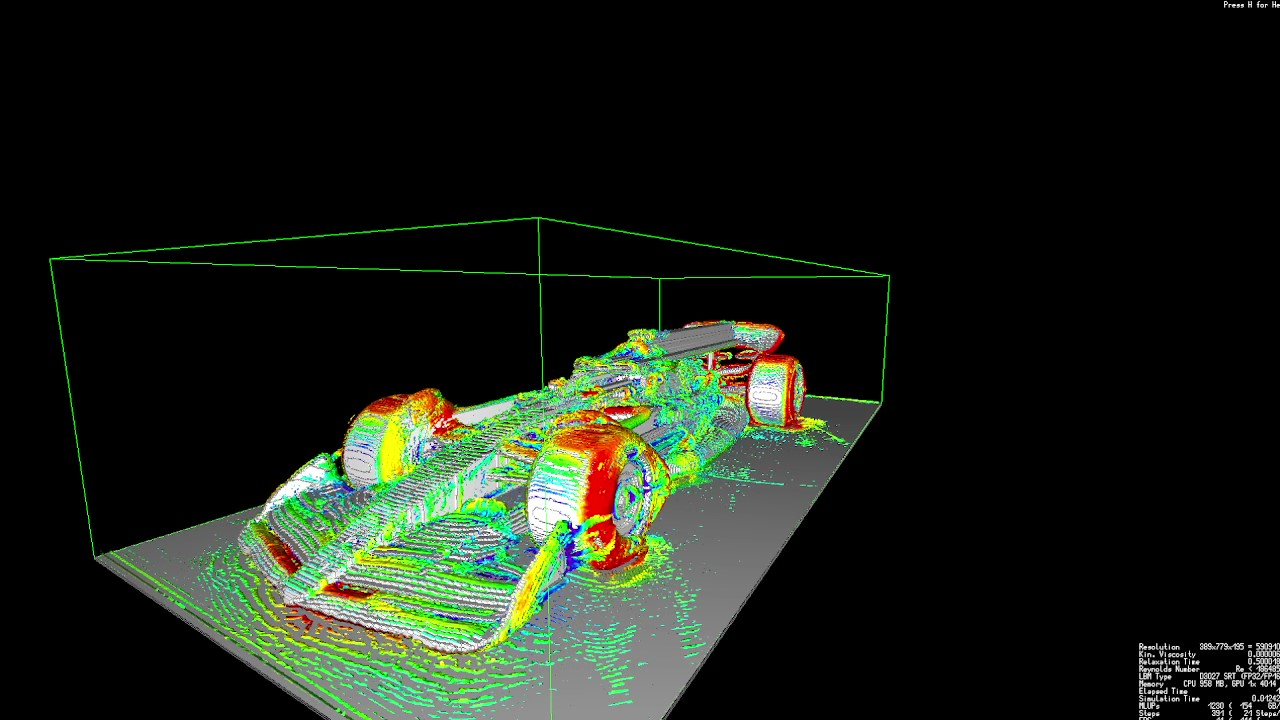
\includegraphics[width=0.9\linewidth]{figures/f1/2023-11-05 13-13-52 - frame at 0m21s.jpg}
            \subcaption{\SI{21}{\second}}
        \end{minipage} \\
        \begin{minipage}[b]{0.45\linewidth}
            \centering
            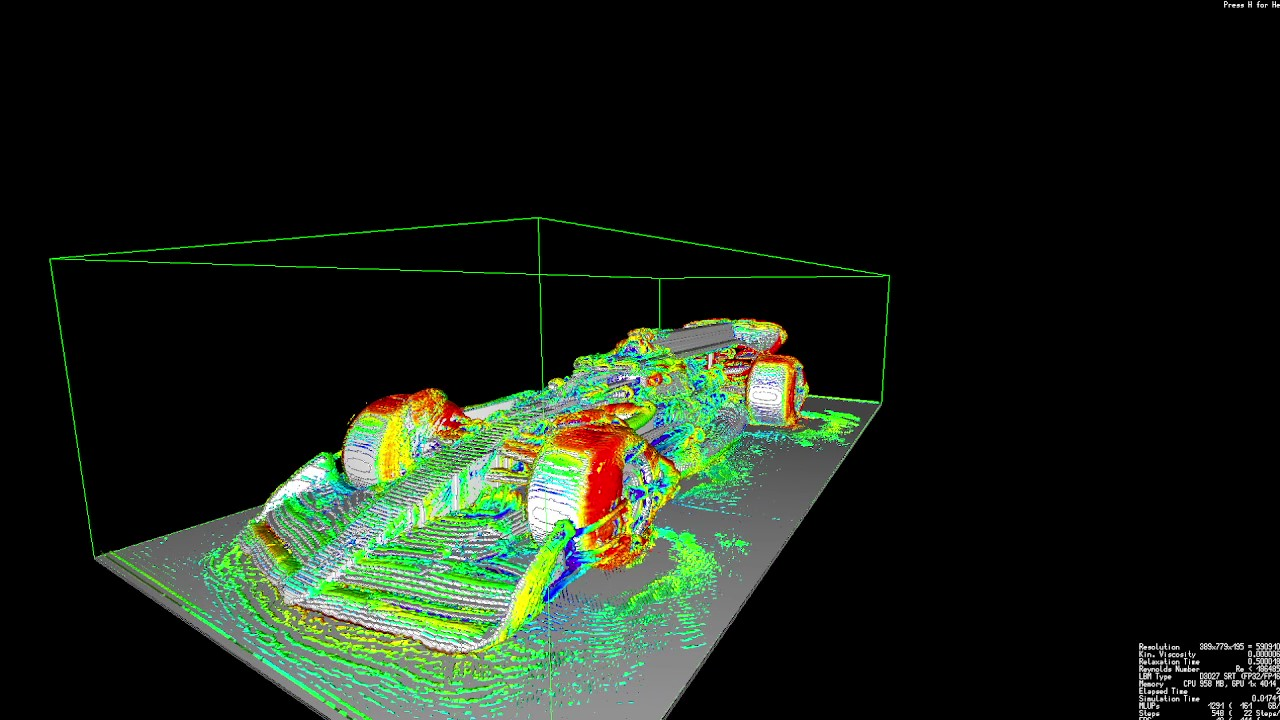
\includegraphics[width=0.9\linewidth]{figures/f1/2023-11-05 13-13-52 - frame at 0m28s.jpg}
            \subcaption{\SI{28}{\second}}
        \end{minipage} &
        \begin{minipage}[b]{0.45\linewidth}
            \centering
            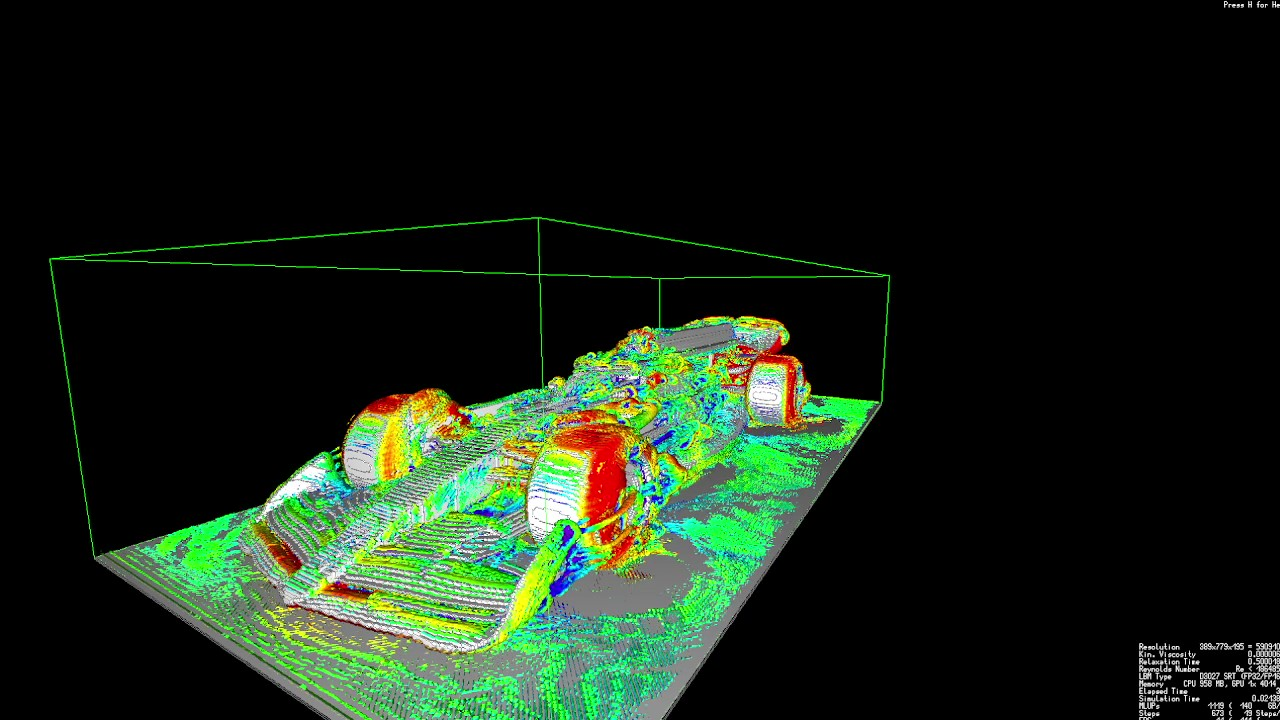
\includegraphics[width=0.9\linewidth]{figures/f1/2023-11-05 13-13-52 - frame at 0m35s.jpg}
            \subcaption{\SI{35}{\second}}
        \end{minipage} \\
        \begin{minipage}[b]{0.45\linewidth}
            \centering
            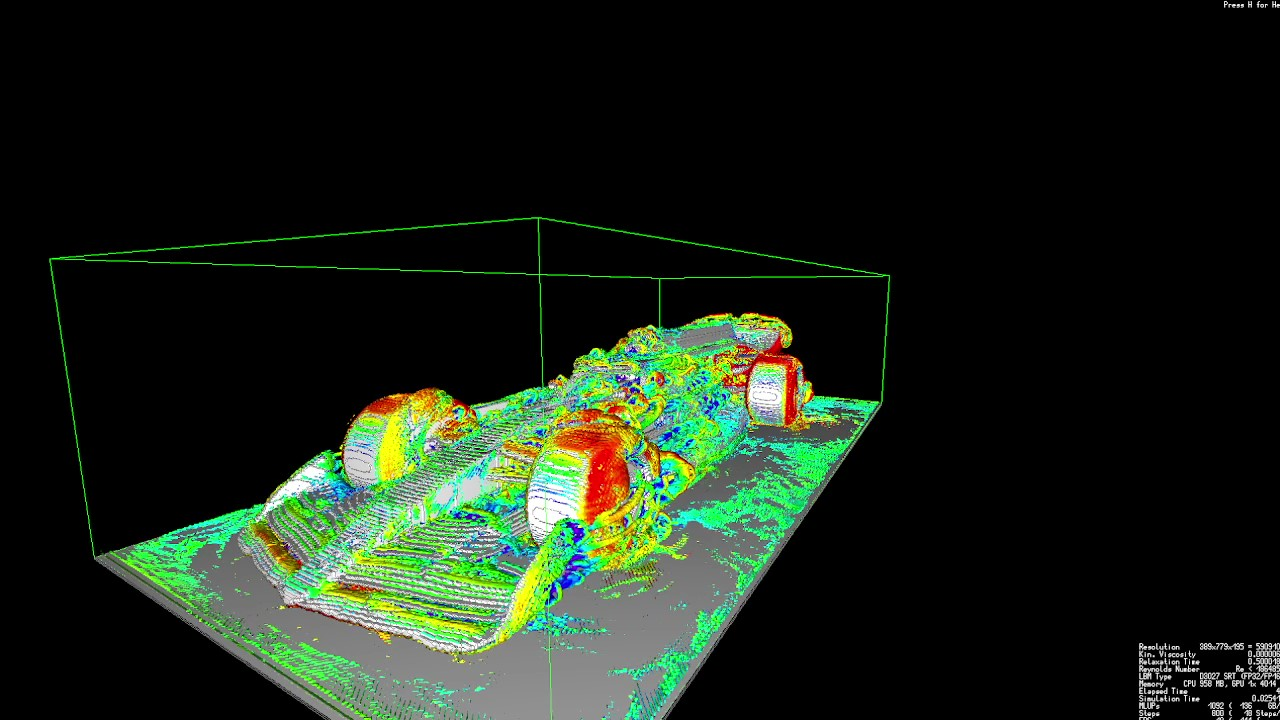
\includegraphics[width=0.9\linewidth]{figures/f1/2023-11-05 13-13-52 - frame at 0m42s.jpg}
            \subcaption{\SI{42}{\second}}
        \end{minipage} &
        \begin{minipage}[b]{0.45\linewidth}
            \centering
            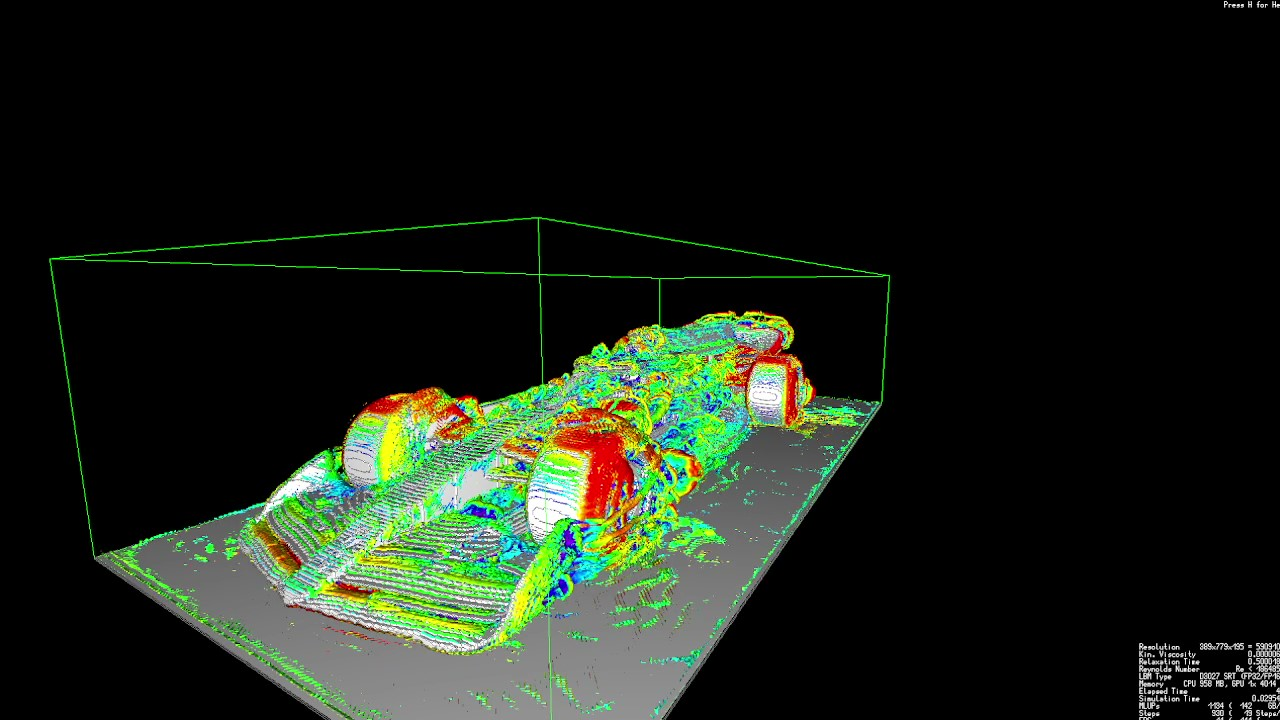
\includegraphics[width=0.9\linewidth]{figures/f1/2023-11-05 13-13-52 - frame at 0m49s.jpg}
            \subcaption{\SI{49}{\second}}
        \end{minipage} \\
        \begin{minipage}[b]{0.45\linewidth}
            \centering
            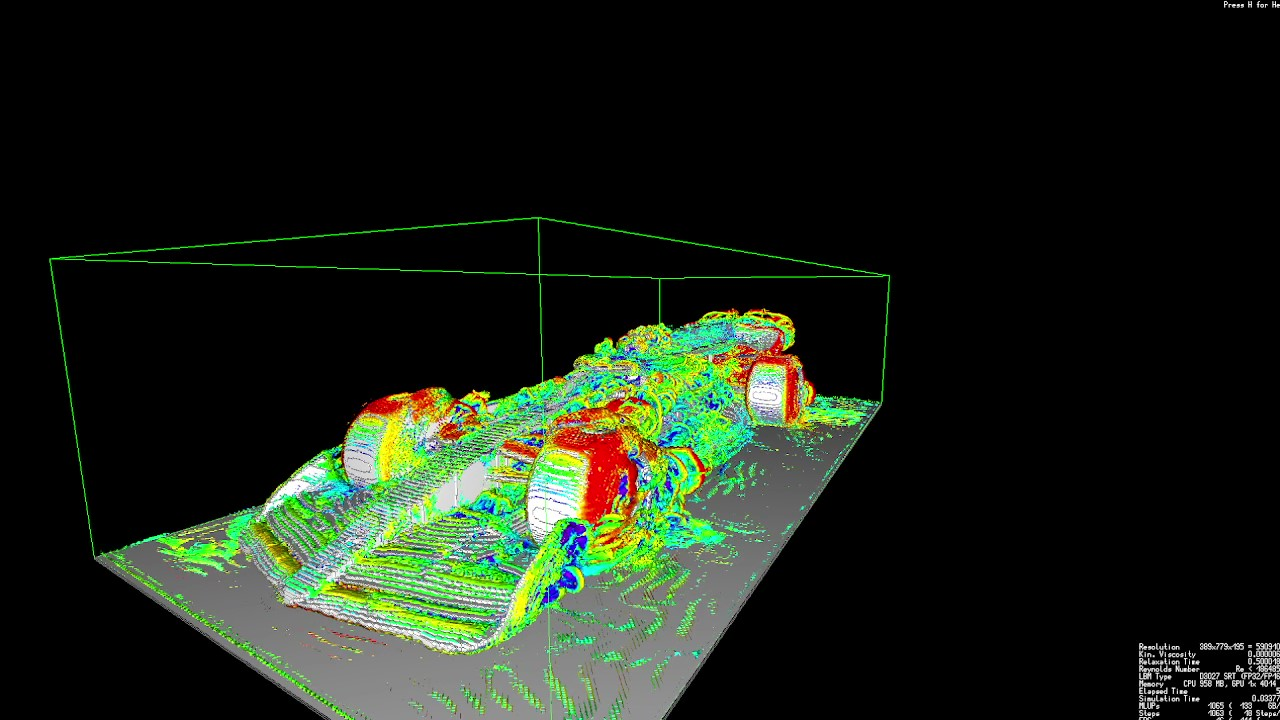
\includegraphics[width=0.9\linewidth]{figures/f1/2023-11-05 13-13-52 - frame at 0m56s.jpg}
            \subcaption{\SI{56}{\second}}
        \end{minipage} &
        \begin{minipage}[b]{0.45\linewidth}
            \centering
            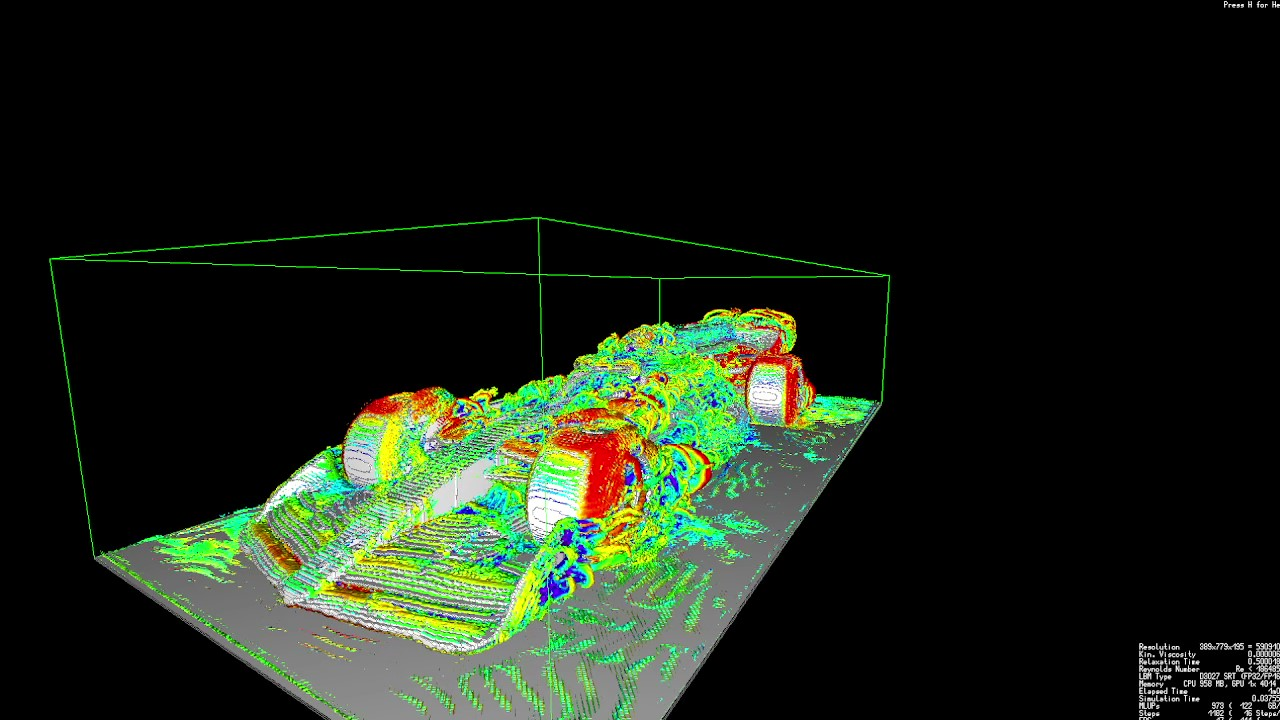
\includegraphics[width=0.9\linewidth]{figures/f1/2023-11-05 13-13-52 - frame at 1m3s.jpg}
            \subcaption{\SI{63}{\second}}
        \end{minipage}
    \end{tabular}

    \caption{Formula1 Mercedes W14の周りの空気の流れ}
    \label{fig:result-f1}
\end{figure}

\subsection{Space Shuttle}
Space Shuttleの周りの気流の様子を図\ref{fig:result-space}に示す.

\begin{figure}[ht]
    \begin{tabular}{cc}
        \begin{minipage}[b]{0.45\linewidth}
            \centering
            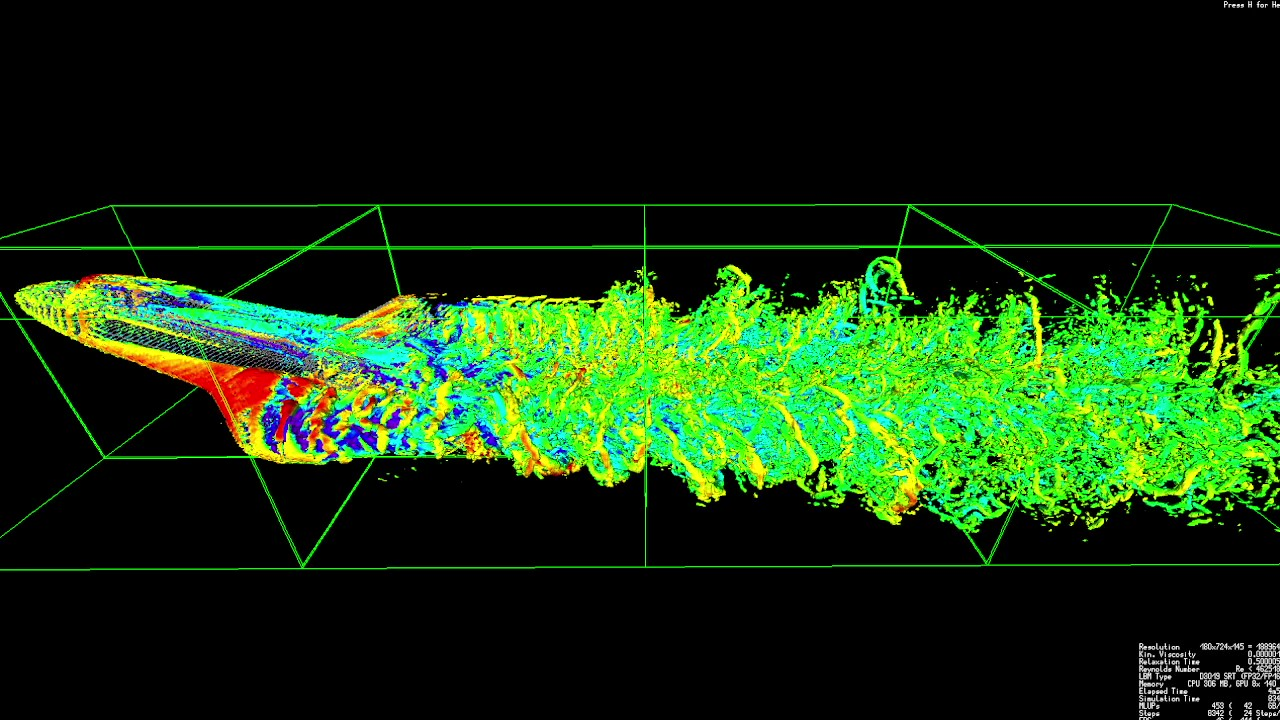
\includegraphics[width=0.9\linewidth]{figures/space/2023-11-05 13-08-17 - frame at 0m0s.jpg}
            \subcaption{\SI{0}{\second}}
        \end{minipage} &
        \begin{minipage}[b]{0.45\linewidth}
            \centering
            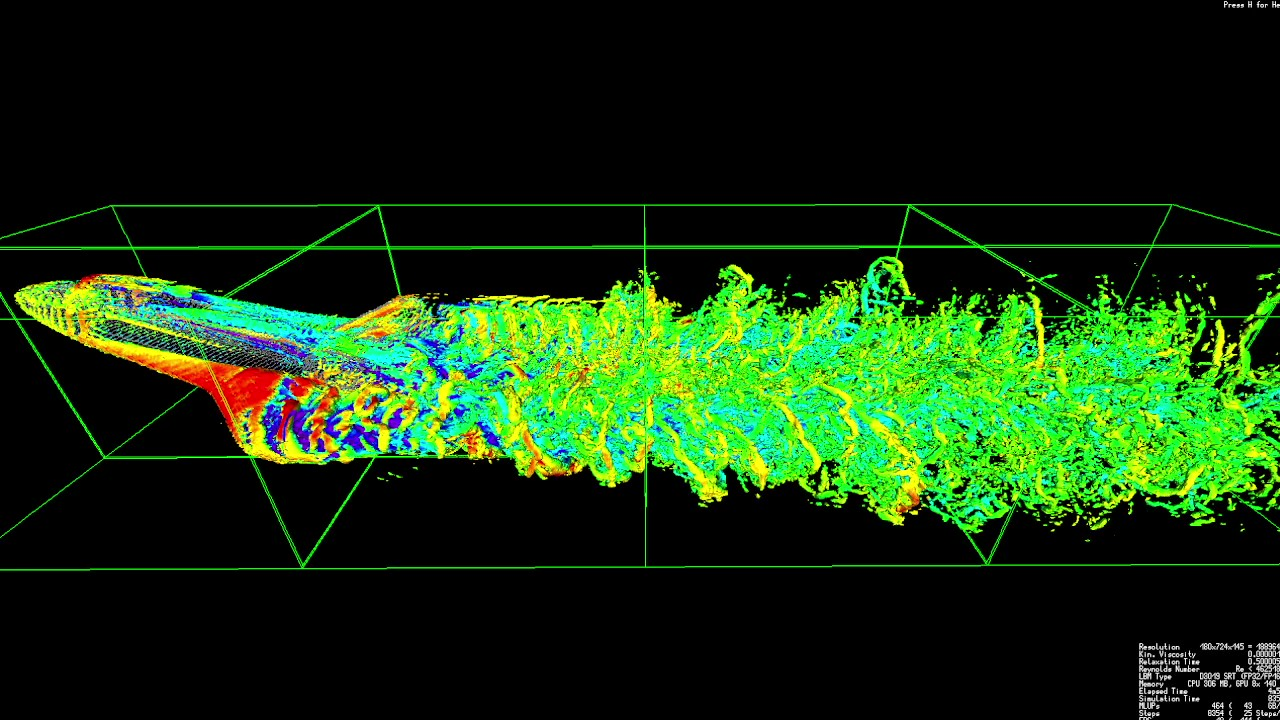
\includegraphics[width=0.9\linewidth]{figures/space/2023-11-05 13-08-17 - frame at 0m1s.jpg}
            \subcaption{\SI{1}{\second}}
        \end{minipage} \\
        \begin{minipage}[b]{0.45\linewidth}
            \centering
            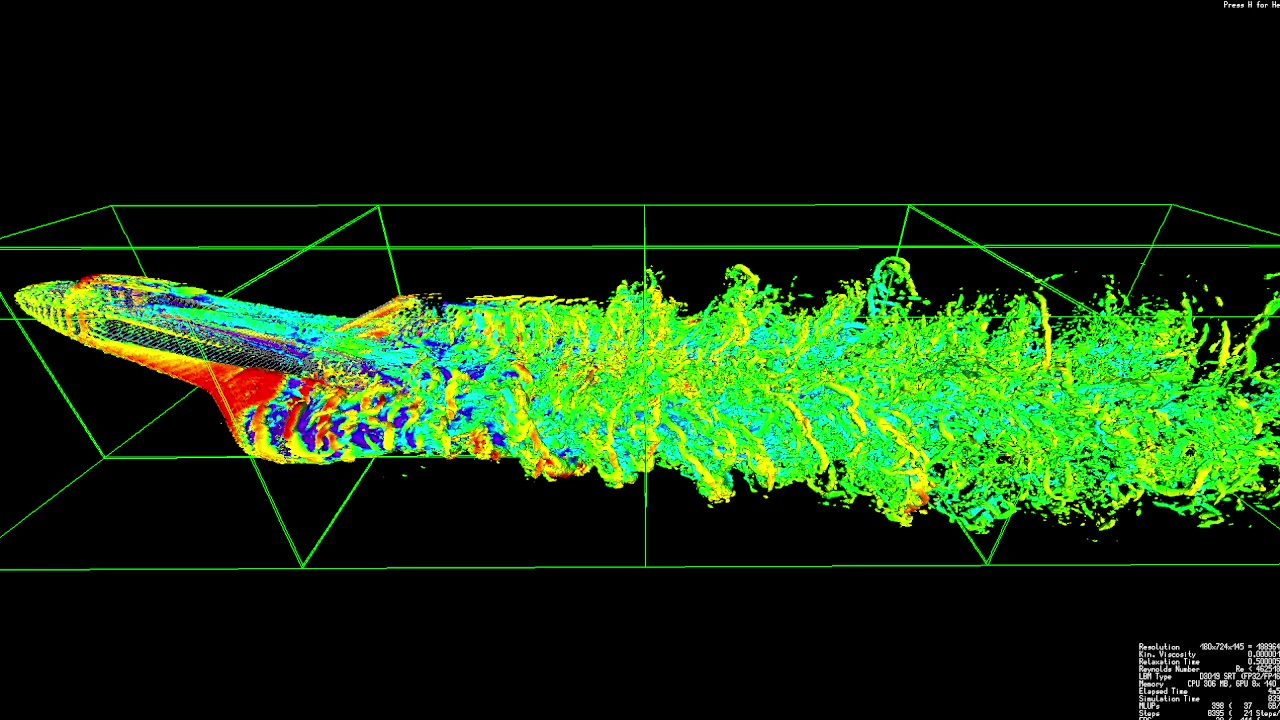
\includegraphics[width=0.9\linewidth]{figures/space/2023-11-05 13-08-17 - frame at 0m2s.jpg}
            \subcaption{\SI{2}{\second}}
        \end{minipage} &
        \begin{minipage}[b]{0.45\linewidth}
            \centering
            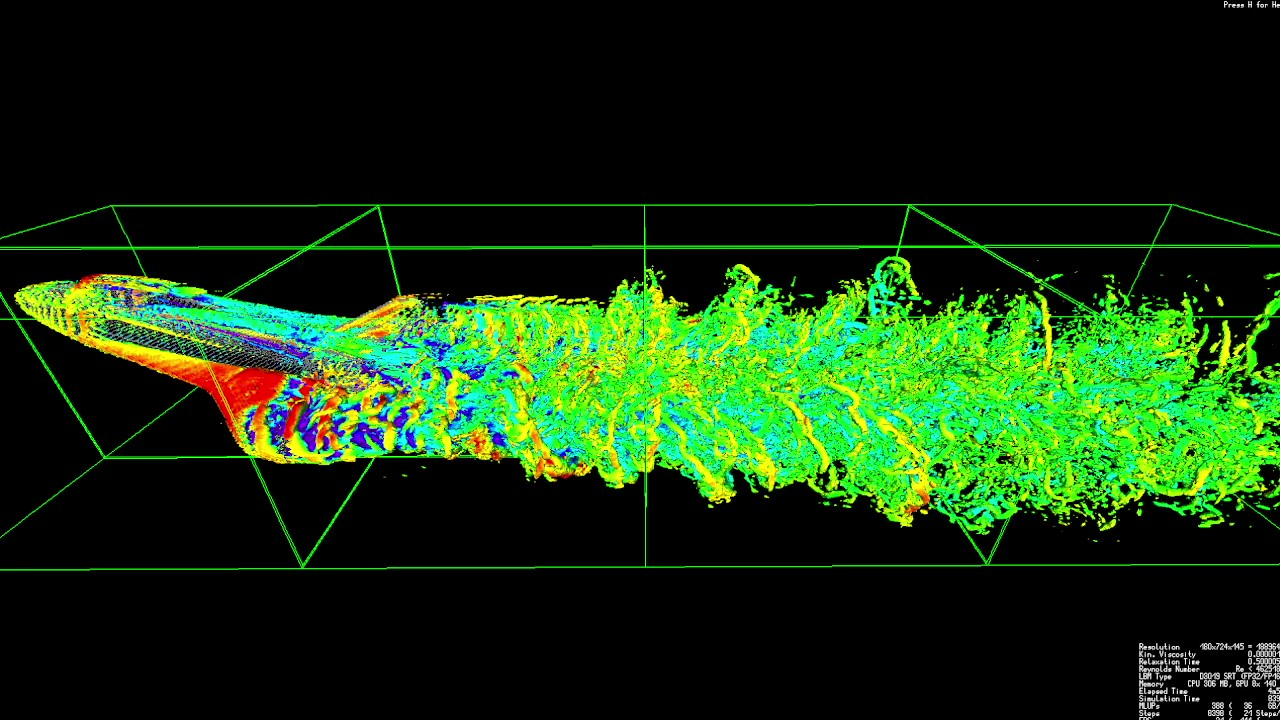
\includegraphics[width=0.9\linewidth]{figures/space/2023-11-05 13-08-17 - frame at 0m3s.jpg}
            \subcaption{\SI{3}{\second}}
        \end{minipage} \\
    \end{tabular}
    \caption{スペースシャトルの周りの気流の様子}
    \label{fig:result-space}
\end{figure}

\subsection{考察}
気流が物体に当たった場所から後方に流れていくにつれてその点を中心に円錐状に広がっていることがわかり,
それらが重なり合って渦が発生しているように見える.
これは原理で述べたように,
LBMでは各格子から後方に行くにつれて隣接する格子にそれぞれ速度や衝突による影響が伝播していくためであると考えられる.

また,F1ではフロントウィングで抵抗がそこまで大きくなく,
それより後方のフロントウィングや後方のリアウィングでの抵抗が大きく赤い部分が見て取れる.
同様にスペースシャトルでも先端部分よりも後方の羽の付け根の部分で抵抗が大きくなっている.
このことから,先端部分では気流を乱さず後方に流し,できる限り後方での抵抗を小さくするように設計されているのではと推察できる.
\footnote{
    しばしば,F1ではフロントウィングはこのような点,すなわち
    ボディの下を通してディヒューザーに流す,ボディの上部からエンジンへ流す,リアウィングへあてる,など
    様々なパーツへと気流を流すために,極めて重要な部品であると言われている.
}

\clearpage

\section{Ahmed Blluff Body}
次に,Ahmed Bluff Bodyと呼ばれる次の図\ref{fig:ahmed-body}のようなモデルを用いて,シミュレーションをした.
このモデルは,CFDのベンチマークとして用いられるモデルであり,
抵抗係数$Cd$,浮力係数$Cl$が次の表\ref{tab:ahmed-cd-cl}のように知られている\cite{ref:ahmed-bluff-body}.
今回は,動せん断粘度$\nu=\SI{2.5E-6}{\square\meter\per\second}$,最大レイノルズ数$Re=5.89E7$,
シミュレーション時間は$\SI{0.25}{\second}$としてシミュレーションをした.

得られた$Cd$の時間変化を図\ref{fig:ahmed-cd-t}に示す.
このうち,$Cd$の値を$0$から$1$までの範囲に限定したものを図\ref{fig:ahmed-cd-t-lim}に示す.

\begin{figure}[ht]
    \begin{minipage}{0.48\linewidth}
        \centering
        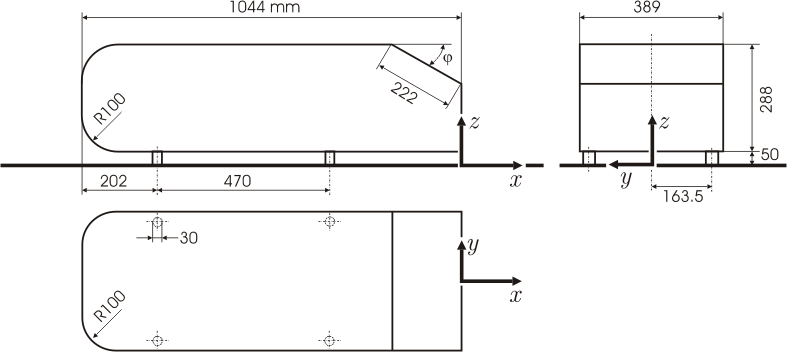
\includegraphics[width=\linewidth]{figures/ahmed/ahmed.png}
        \subcaption{設計図}
    \end{minipage}
    \begin{minipage}{0.48\linewidth}
        \centering
        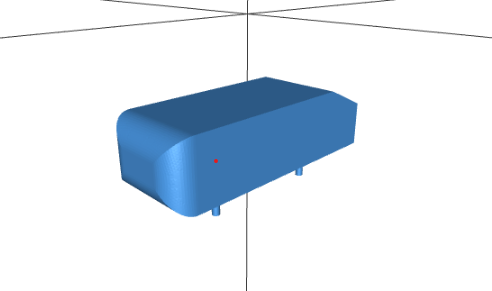
\includegraphics[width=\linewidth]{figures/ahmed/img.png}
        \subcaption{外観}
    \end{minipage}
    \caption{Ahmed Bluff Body}
    \label{fig:ahmed-body}
\end{figure}

\begin{table}[htbp]
    \centering
    \caption{Ahmed Bluff Bodyの抵抗係数$Cd$,浮力係数$Cl$}
    \begin{tabular}{ccc}
        \toprule
           & Cd    & Cl    \\
        \midrule
           & 0.300 & 0.316 \\
           & 0.266 & 0.325 \\
           & 0.274 & 0.33  \\
           & 0.250 & 0.306 \\
           & 0.260 & 0.305 \\
           & 0.301 & 0.307 \\
        \midrule
        平均 & 0.275 & 0.315 \\
        \bottomrule
    \end{tabular}%
    \label{tab:ahmed-cd-cl}%
\end{table}%

\begin{figure}[ht]
    \centering
    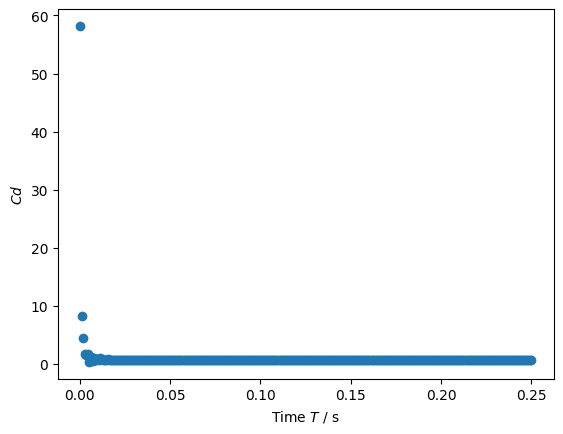
\includegraphics[width=0.8\linewidth]{figures/ahmed/ahmed-cd.png}
    \caption{AhmedBluffBodyの$Cd$の時間変化}\label{fig:ahmed-cd-t}
\end{figure}

\begin{figure}[ht]
    \centering
    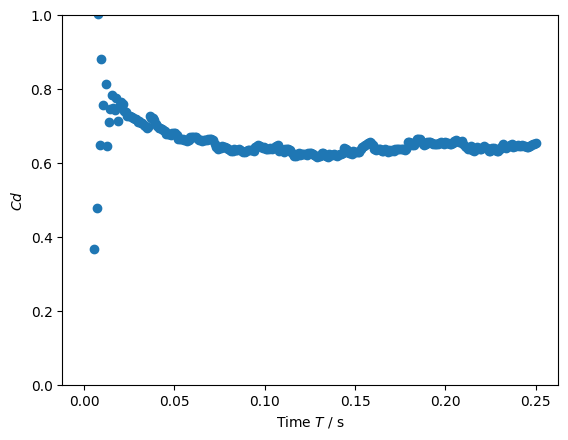
\includegraphics[width=0.8\linewidth]{figures/ahmed/ahmed-cd-0-1.png}
    \caption{AhmedBluffBodyの$Cd$の時間変化 拡大図}\label{fig:ahmed-cd-t-lim}
\end{figure}
\subsection{考察}
$Cd$の値は,図\ref{fig:ahmed-cd-t}から,
\SI{0.1}{\second}以降は\SI{0.63}{}から\SI{0.66}{}の間で推移している.
この値は,表\ref{tab:ahmed-cd-cl}の値と比較すると,約\SI{2}{}倍程度大きい.
このことから,FluidX3Dのシミュレーションでは実際の値よりも抵抗が大きくなっており,
その原因として考えられることは,衝突による計算アルゴリズムが適当ではないということがある.

また,図\ref{fig:ahmed-cd-t-lim}より,\SI{0.1}{\second}以降$Cd$が周期的に振動しているように見える.
そこで,\SI{0.1}{\second}以降の$Cd$の値を取り出し,Fourier解析をした.
サンプリング周期を\SI{0.001}{\second},サンプル数を\SI{250}としてFFTを実行すると,振幅スペクトルは
図\ref{fig:ahmed-cd-fft}のようになった.
\SI{4}{\Hz}の振幅がもっとも大きく,その値は\SI{0.09}{}である.
これは$Cd$の時間変化が\SI{0.15}{\second}の間のみであるから,特に意味のない値であると考えらえる.
その次に大きい値は,\SI{12.5}{\Hz}であり,そのときの振幅は\SI{0.047}{}である.
このとき,周期が\SI{0.08}{\second}で周期性があると考えられる.


\begin{figure}
    \centering
    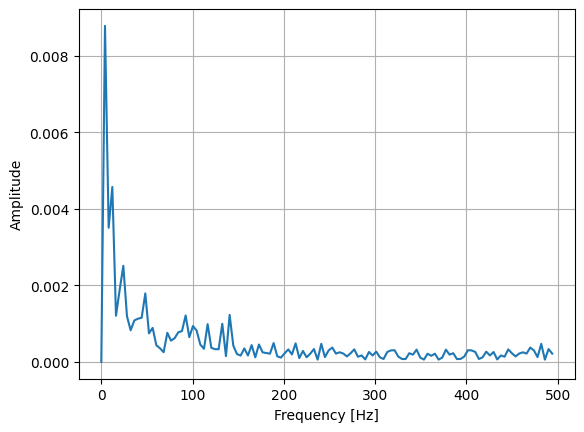
\includegraphics[width=0.8\linewidth]{figures/ahmed/cd-fourier-amplitude.png}
    \caption{AhmedBluffBodyの$Cd$の振幅スペクトル}\label{fig:ahmed-cd-fft}
\end{figure}

\end{document}